% figure: 自控-结构图等效变换规则.png
% 用途：自控 02-3 §2.3.2 —— 结构图等效变换六条规则（串联/并联/反馈 + 比较点·引出点前后移）
% 构建：..\build.ps1 -File .\block-transform-rules.tex
% 记号约定：红色只表示"移动后新增的补偿支路"，以及被移动的求和点/引出点本身；
%          原来的前向信号线一律保持黑色，不改颜色。
\documentclass[border=8pt]{standalone}
\usepackage{fontspec}
\setmainfont{Cambria}
\usepackage{unicode-math}
\setmathfont{Cambria Math}
\usepackage{tikz}
\usetikzlibrary{positioning, arrows.meta, calc}
\usepackage{ctex}

\definecolor{figink}{HTML}{1E2228}
\definecolor{figacc}{HTML}{B23020}
\definecolor{figsub}{HTML}{606874}
\definecolor{figfill}{HTML}{E8EFF8}

\begin{document}
\begin{tikzpicture}[
  x=1cm, y=1cm,
  line width=0.9pt, line cap=round, line join=round,
  >=Stealth,
  blk/.style   = {draw=figink, line width=0.9pt, fill=figfill,
                  minimum width=1.05cm, minimum height=0.62cm, inner sep=1pt,
                  anchor=center, font=\small},
  sum/.style   = {draw=figink, line width=0.9pt, circle, inner sep=0pt,
                  minimum size=0.38cm, anchor=center},
  sumacc/.style = {draw=figacc, line width=0.9pt, circle, inner sep=0pt,
                  minimum size=0.38cm, anchor=center},
  lbl/.style   = {font=\small, inner sep=1.5pt},
  sig/.style   = {font=\small, color=figink},
  comp/.style  = {draw=figacc, line width=0.9pt, fill=white,
                  minimum width=0.9cm, minimum height=0.62cm, inner sep=1pt,
                  anchor=center, font=\small, text=figacc},
  br/.style    = {draw=figacc, line width=0.9pt, ->},
  ctl/.style   = {font=\small\bfseries, color=figink, anchor=north west},
  figcap/.style = {font=\footnotesize, color=figsub, anchor=west},
  toarrow/.style = {draw=figsub, line width=1pt, ->}
]

% ================= 规则 1：串联 =================
\node[ctl] at (-0.6,0.6) {① 串联};
\begin{scope}[shift={(0.8,0)}]
  \draw[->] (0,0) -- (1.0,0);
  \node[blk] (g1) at (1.55,0) {$G_1$};
  \draw[->] (2.10,0) -- (3.0,0);
  \node[blk] (g2) at (3.55,0) {$G_2$};
  \draw[->] (4.10,0) -- (5.1,0);
\end{scope}
\draw[toarrow] (6.2,0) -- (7.1,0);
\node[figcap] at (6.25,0.35) {等价};
\begin{scope}[shift={(7.7,0)}]
  \draw[->] (0,0) -- (1.0,0);
  \node[blk, minimum width=1.6cm] (g) at (1.85,0) {$G_1G_2$};
  \draw[->] (2.70,0) -- (3.6,0);
\end{scope}

% ================= 规则 2：并联 =================
\node[ctl] at (-0.6,-3.0) {② 并联};
\begin{scope}[shift={(0.8,-3.6)}]
  \coordinate (jin) at (0,0);
  \coordinate (jout) at (4.7,0);
  \fill (jin) circle (1.6pt);
  \fill (jout) circle (1.6pt);
  \node[blk] (ga) at (2.1,0.75) {$G_1$};
  \node[blk] (gb) at (2.1,-0.75) {$G_2$};
  \draw[->] (jin) -- (0.7,0) |- (ga.west);
  \draw[->] (jin) -- (0.7,0) |- (gb.west);
  \draw[->] (ga.east) -| (jout);
  \draw[->] (gb.east) -| (jout);
  \draw[->] (jout) -- (5.5,0);
\end{scope}
\draw[toarrow] (6.2,-3.6) -- (7.1,-3.6);
\node[figcap] at (6.25,-3.25) {等价};
\begin{scope}[shift={(7.7,-3.6)}]
  \draw[->] (0,0) -- (0.85,0);
  \node[blk, minimum width=1.8cm] (g) at (1.75,0) {$G_1\pm G_2$};
  \draw[->] (2.65,0) -- (3.55,0);
\end{scope}

% ================= 规则 3：反馈 =================
\node[ctl] at (-2.3,-6.6) {③ 反馈};
\begin{scope}[shift={(2.0,-7.0)}]
  \node[sum] (s1) at (0,0) {};
  \node[blk] (g) at (1.75,0) {$G$};
  \draw[->] (-1.0,0) -- (s1.west);
  \draw[->] (s1.east) -- (g.west);
  \draw[->] (g.east) -- (3.4,0);
  \draw[->] (2.7,0) -- (2.7,-1.3) -- (0,-1.3) -- (s1.south);
  \node[blk] (h) at (1.35,-1.3) {$H$};
  \node[lbl] at (-0.34,0.30) {$+$};
  \node[lbl] at (-0.44,-0.30) {$-$};
\end{scope}
\draw[toarrow] (6.2,-7.0) -- (7.1,-7.0);
\node[figcap] at (6.25,-6.65) {等价};
\begin{scope}[shift={(7.7,-7.0)}]
  \draw[->] (0,0) -- (0.85,0);
  \node[blk, minimum width=1.9cm] (phi) at (1.85,0) {$\dfrac{G}{1\pm GH}$};
  \draw[->] (2.85,0) -- (3.75,0);
\end{scope}

% ================= 规则 4：比较点前移 =================
\node[ctl] at (-0.6,-10.0) {④ 比较点前移};
\begin{scope}[shift={(0.8,-10.4)}]
  \coordinate (X1) at (1.05,0);
  \node[sum] (s1) at (2.05,0) {};
  \node[blk] (g1) at (3.65,0) {$G_1$};
  \draw[->] (-0.4,0) -- (1.86,0);
  \draw[->] (X1) -- (1.05,-0.85) -- (3.65,-0.85) -- (3.65,-0.31);
  \node[sig] at (0.88,0.28) {$X_1$};
  \draw[->] (s1.east) -- node[sig, above] {$X_2$} (g1.west);
  \draw[->] (g1.east) -- (4.7,0);
  \node[lbl] at (1.76,0.30) {$+$};
  \node[lbl] at (2.05,-0.44) {$-$};
  \fill (X1) circle (1.6pt);
\end{scope}
\draw[toarrow] (6.2,-10.4) -- (7.1,-10.4);
\node[figcap] at (6.25,-10.05) {等价};
\begin{scope}[shift={(7.7,-10.4)}]
  \coordinate (X1) at (0.95,0);
  \node[blk] (g1) at (2.45,0) {$G_1$};
  \coordinate (X2) at (3.5,0);
  \node[sumacc] (s1) at (4.55,0) {};
  \node[comp] (c) at (5.75,-1.35) {$\dfrac{1}{G_1}$};
  % 前向支路：输入 -> G1 -> X2 停止；X2 之后的信号由补偿支路反送回比较点
  \draw[->] (X1) -- (g1.west);
  \draw[->] (g1.east) -- (X2);
  \node[sig] at (0.72,0.30) {$X_1$};
  \node[sig] at (3.42,0.34) {$X_2$};
  \draw[->] (s1.east) -- (6.2,0);
  % 补偿支路：由移动后的比较点位置引出，经 1/G1 送回
  \draw[br] (X2) -- (X2 |- 0,-1.35) -- (c.east);
  \draw[br] (c.west) -- (4.55,-1.35) -- (s1.south);
  \node[lbl] at (4.36,0.30) {$+$};
  \node[lbl] at (4.55,-0.44) {$-$};
  \fill[figacc] (X2) circle (1.9pt);
  \fill[figacc] (s1.north) circle (1.9pt);
\end{scope}

% ================= 规则 5：引出点前移 =================
\node[ctl] at (-0.6,-13.4) {⑤ 引出点前移};
\begin{scope}[shift={(0.8,-13.8)}]
  \node[blk] (g1) at (2.1,0) {$G_1$};
  \coordinate (X2) at (3.35,0);
  \draw[->] (-0.4,0) -- (g1.west);
  \draw[->] (g1.east) -- (4.6,0);
  \node[sig] at (1.45,0.28) {$X_1$};
  \draw[->] (X2) -- (3.35,1.25) -- (4.6,1.25);
  \node[sig] at (3.5,0.28) {$X_2$};
  \fill (X2) circle (1.6pt);
\end{scope}
\draw[toarrow] (6.2,-13.8) -- (7.1,-13.8);
\node[figcap] at (6.25,-13.45) {等价};
\begin{scope}[shift={(7.7,-13.8)}]
  \coordinate (X1) at (0.9,0);
  \node[blk] (g1) at (2.5,0) {$G_1$};
  \draw[->] (X1) -- (g1.west);
  \draw[->] (g1.east) -- (4.9,0);
  \node[sig] at (1.85,0.30) {$X_1$};
  % 移动后的引出点（红点）与串入的 1/G1 补偿支路
  \fill[figacc] (X1) circle (1.9pt);
  \node[comp] (c) at (2.5,1.35) {$\dfrac{1}{G_1}$};
  \draw[br] (X1) -- (X1 |- 0,1.35) -- (c.west);
  \draw[br] (c.east) -- (4.9,1.35);
\end{scope}

% ================= 规则 6：引出点后移 =================
\node[ctl] at (-0.6,-16.8) {⑥ 引出点后移};
% before：引出点在方框之前
\begin{scope}[shift={(0.8,-17.2)}]
  \coordinate (X1) at (0.9,0);
  \node[blk] (g1) at (2.5,0) {$G_1$};
  \draw[->] (X1) -- (g1.west);
  \draw[->] (g1.east) -- (4.9,0);
  \fill (X1) circle (1.6pt);
  \node[sig] at (1.5,0.28) {$X_1$};
  \draw[->] (X1) -- (0.9,1.35) -- (4.9,1.35);
\end{scope}
\draw[toarrow] (6.2,-17.2) -- (7.1,-17.2);
\node[figcap] at (6.25,-16.85) {等价};
% after：引出点移到方框之后，引出支路需串入 G1
\begin{scope}[shift={(7.7,-17.2)}]
  \node[blk] (g1) at (2.1,0) {$G_1$};
  \coordinate (X2) at (3.6,0);
  \draw[->] (0,0) -- (g1.west);
  \draw[->] (g1.east) -- (4.9,0);
  \fill[figacc] (X2) circle (1.9pt);
  \node[sig] at (3.72,0.30) {$X_2$};
  \node[comp] (c) at (4.45,1.35) {$G_1$};
  \draw[br] (X2) -- (X2 |- 0,1.35) -- (c.west);
  \draw[br] (c.east) -- (5.9,1.35);
\end{scope}

\end{tikzpicture}
\end{document}
